\documentclass{beamer}
\usepackage[utf8]{inputenc}
\usepackage{tikz}
\usetikzlibrary{shapes.geometric, arrows}
\tikzstyle{std} = [rectangle, minimum width=7cm, minimum height=0.8cm, text centered, align = center, draw=black, fill=gray!30] 
\tikzstyle{arrow} = [->,>=stealth]
\addtobeamertemplate{navigation symbols}{}{%
    \usebeamerfont{footline}%
    \usebeamercolor[fg]{footline}%
    \hspace{1em}%
    \insertframenumber/\inserttotalframenumber
  }

%Information to be included in the title page:
\title{Competition and Idoelogical Diversity: Historical Evidence from US Newspapers}
\author{Caio Figueiredo}
\institute{Penn State}
\date{2019}
 
\begin{document}
 
\frame{\titlepage}
 
\begin{frame}
  \frametitle{Introduction}
  \begin{itemize}
    \item Objective: Formulate a model of newspaper demand, entry, and political affiliation choice.
  \end{itemize}

\end{frame}

\begin{frame}[t]{Context}
  \begin{itemize}
    \item The year is 1924.
    \item (Most) newspapers openly declare political affiliation.
    \item There is no TV and Radio is at its infancy. Which for us means 
      that the outside option is "No News", simplifying treatment.
  \end{itemize}
\end{frame}

\begin{frame}[t]{Model Sketch}
  \center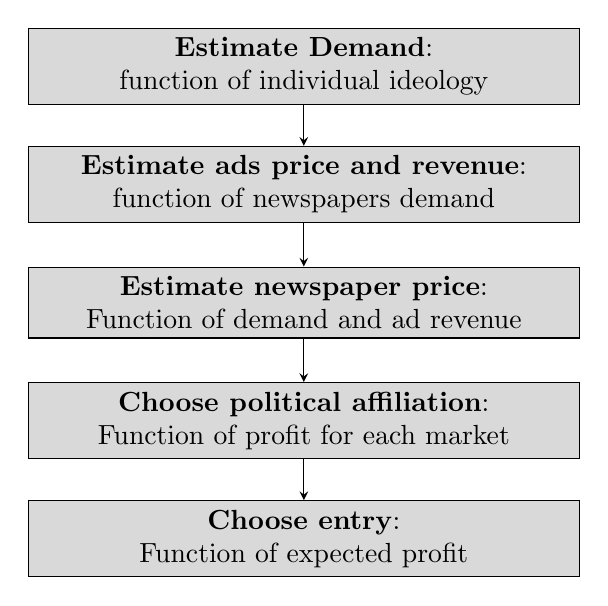
\begin{tikzpicture}[baseline=0, node distance=1.5cm]
    \node (demand) [std, align=center]    
      {\textbf{Estimate Demand}: \\ function of individual ideology};
    \node (ads)    [std, below of=demand] 
      {\textbf{Estimate ads price and revenue}: \\ function of newspapers 
        demand};
    \node (price)  [std, below of=ads]   
      {\textbf{Estimate newspaper price}: \\ Function of demand and ad revenue};
    \node (ideo)   [std, below of=price] 
      {\textbf{Choose political affiliation}: \\ Function of profit for each 
        market};
    \node (entry)  [std, below of=ideo]  
      {\textbf{Choose entry}: \\ Function of expected profit};

    \draw [arrow] (demand) -- (ads);
    \draw [arrow] (ads)    -- (price);
    \draw [arrow] (price)  -- (ideo);
    \draw [arrow] (ideo)   -- (entry);
  \end{tikzpicture}
\end{frame}

\begin{frame}[t]{Data}
  \begin{itemize}
    \item For the supply side (Entry and affiliation), data on the number,
      affiliations, and circulation prices of individual newspaper are used.
      \item Collected from the US Newspaper Panel
    \item Vote share is used as proxy of consumers political affiliation.
    \item For the demand side, data on circulation per town and newspaper
      is used.
      \item Collect from Audit Bureau of Circulations.
    \item Supplementary datasets on newspaper revenue and costs, alongside 
      readership surveys, are used to calibrate the model
    \item \textit{Note: The process of matching data from the different databases
      is complex and a considerable ammount of data is lost.}
  \end{itemize}
\end{frame}

\begin{frame}[t]{Data Summary for markets - US Newspaper Panel}
  \begin{figure}
  \begin{center}
    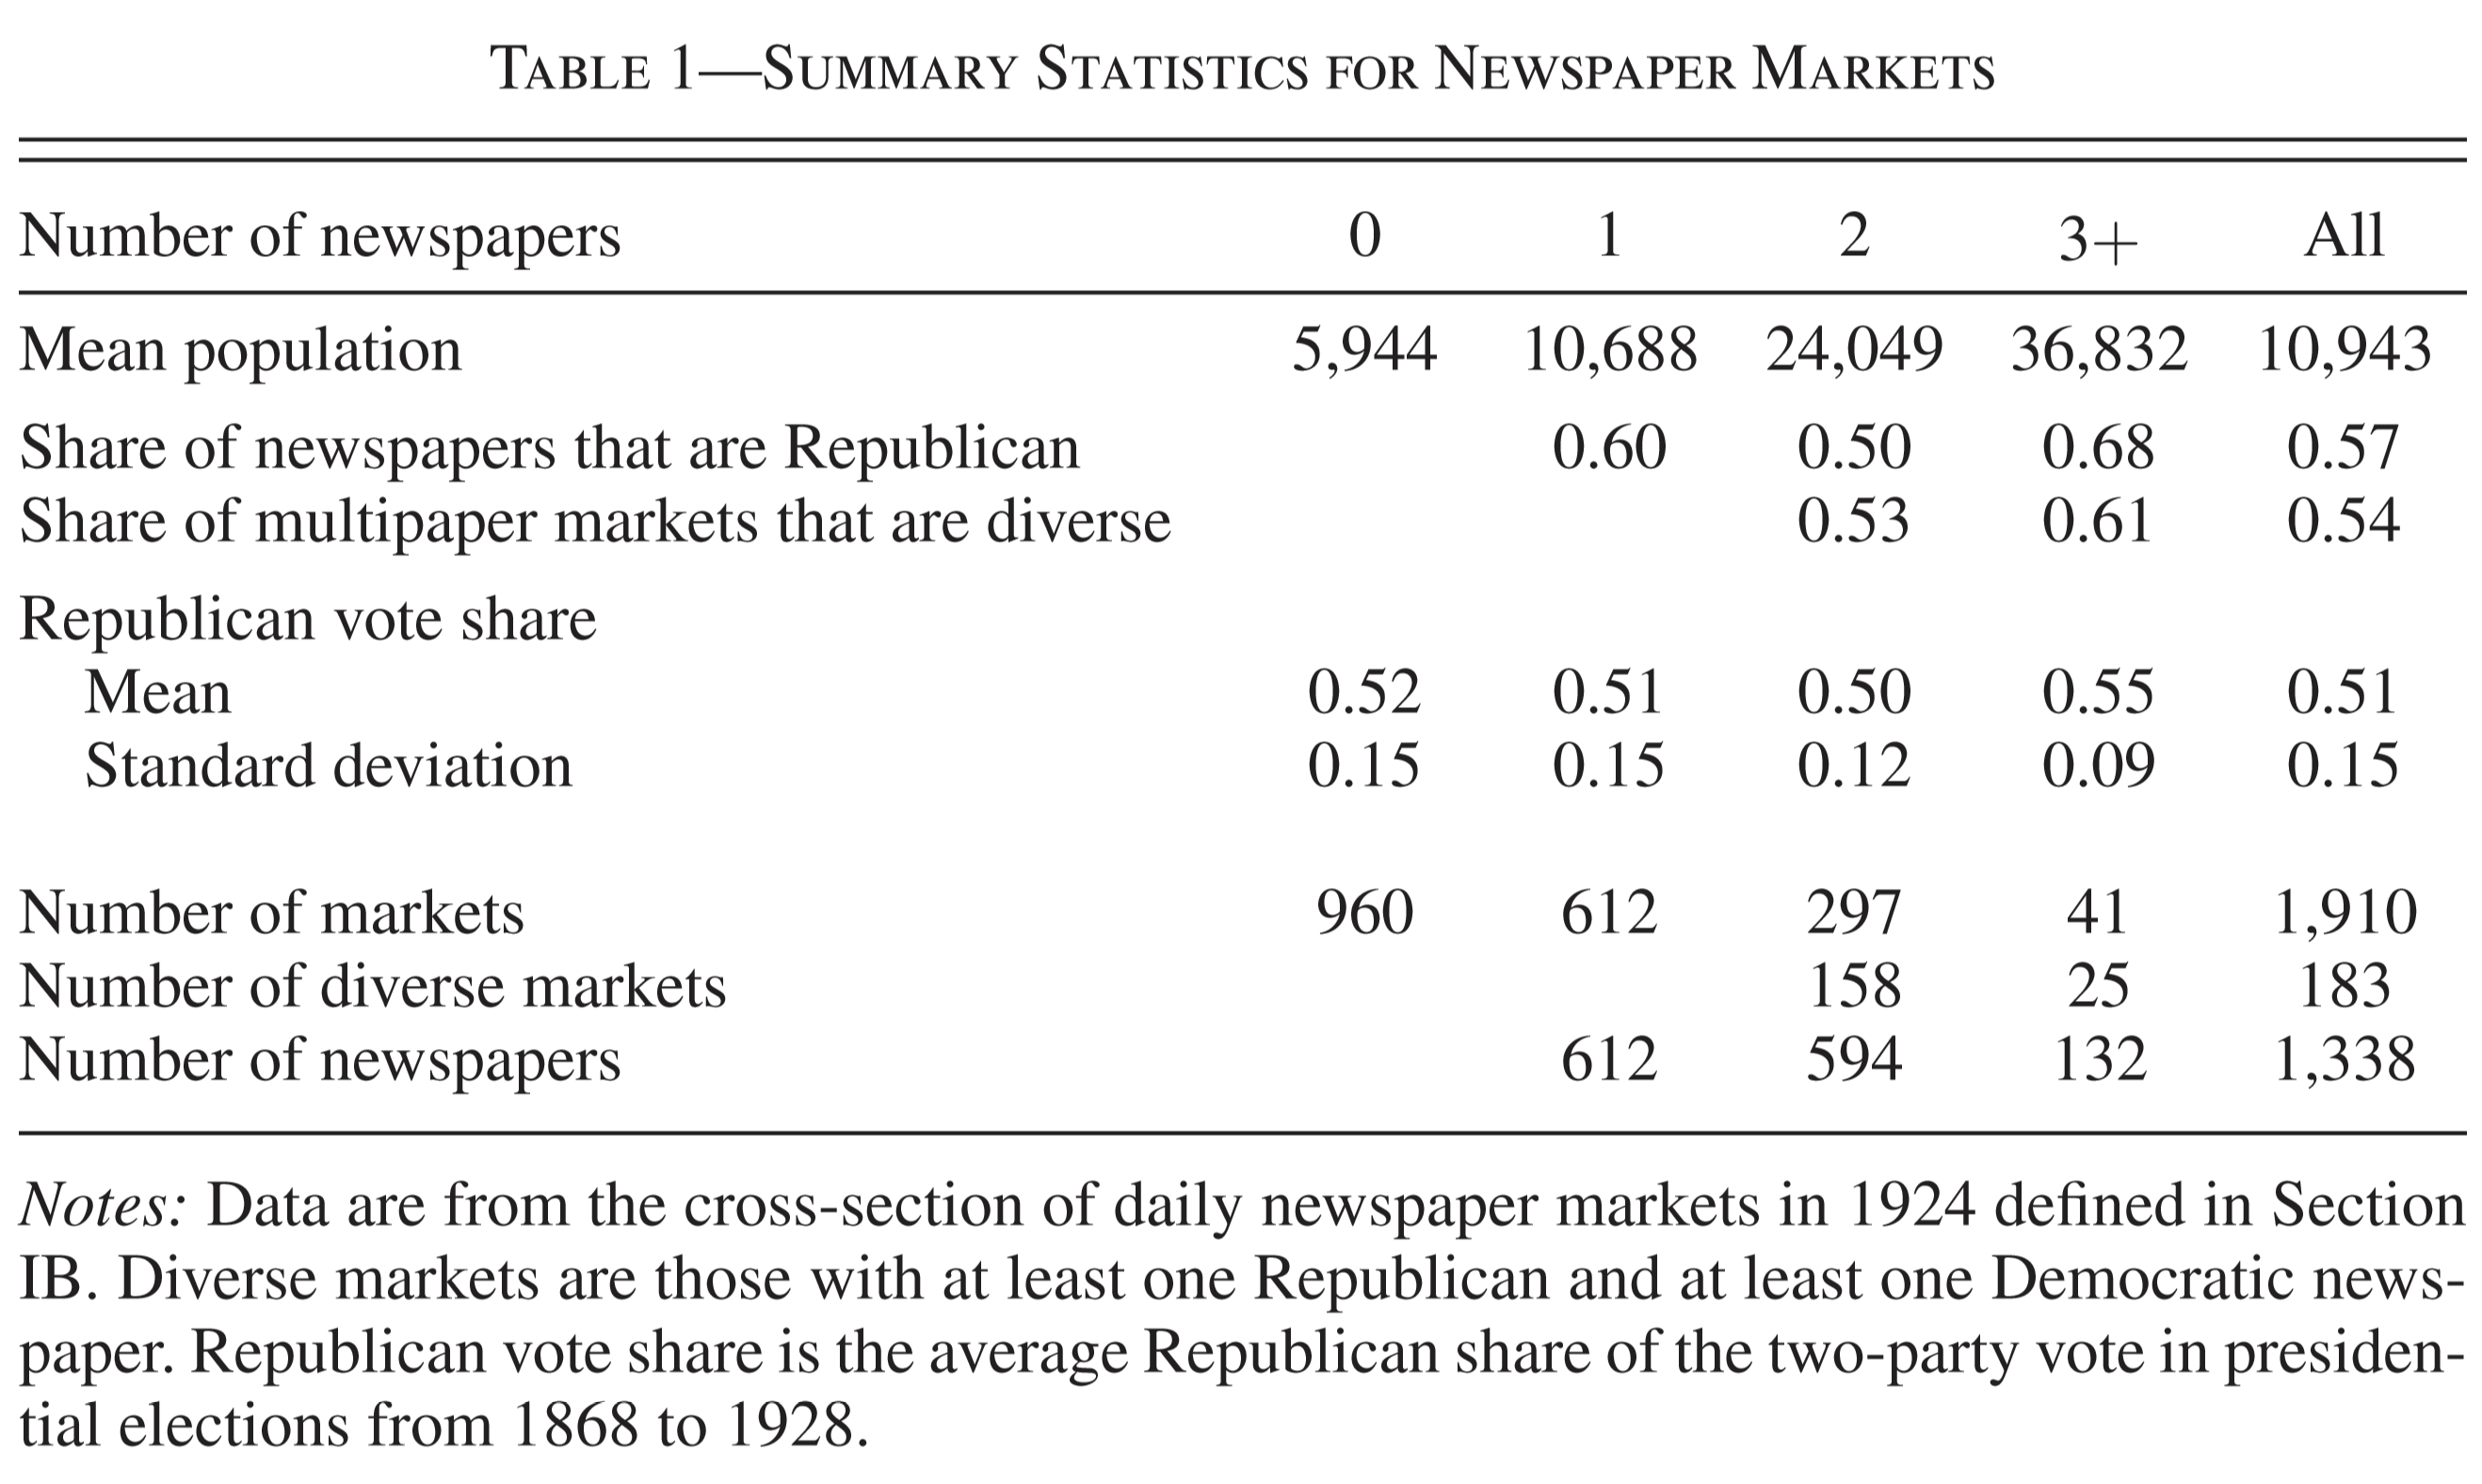
\includegraphics[scale=0.14]{Table1.png}
  \end{center}
  \end{figure}

  \begin{itemize}
    \item Number of papers is highly correlated to population
    \item The share of Republican Newspapers (57\%) is slightly higher than
      the share of Republican votes (51\%)
  \end{itemize}
\end{frame}

\begin{frame}[t]{Data Summary for towns - ABC x Panel}
  \begin{figure}
  \begin{center}
    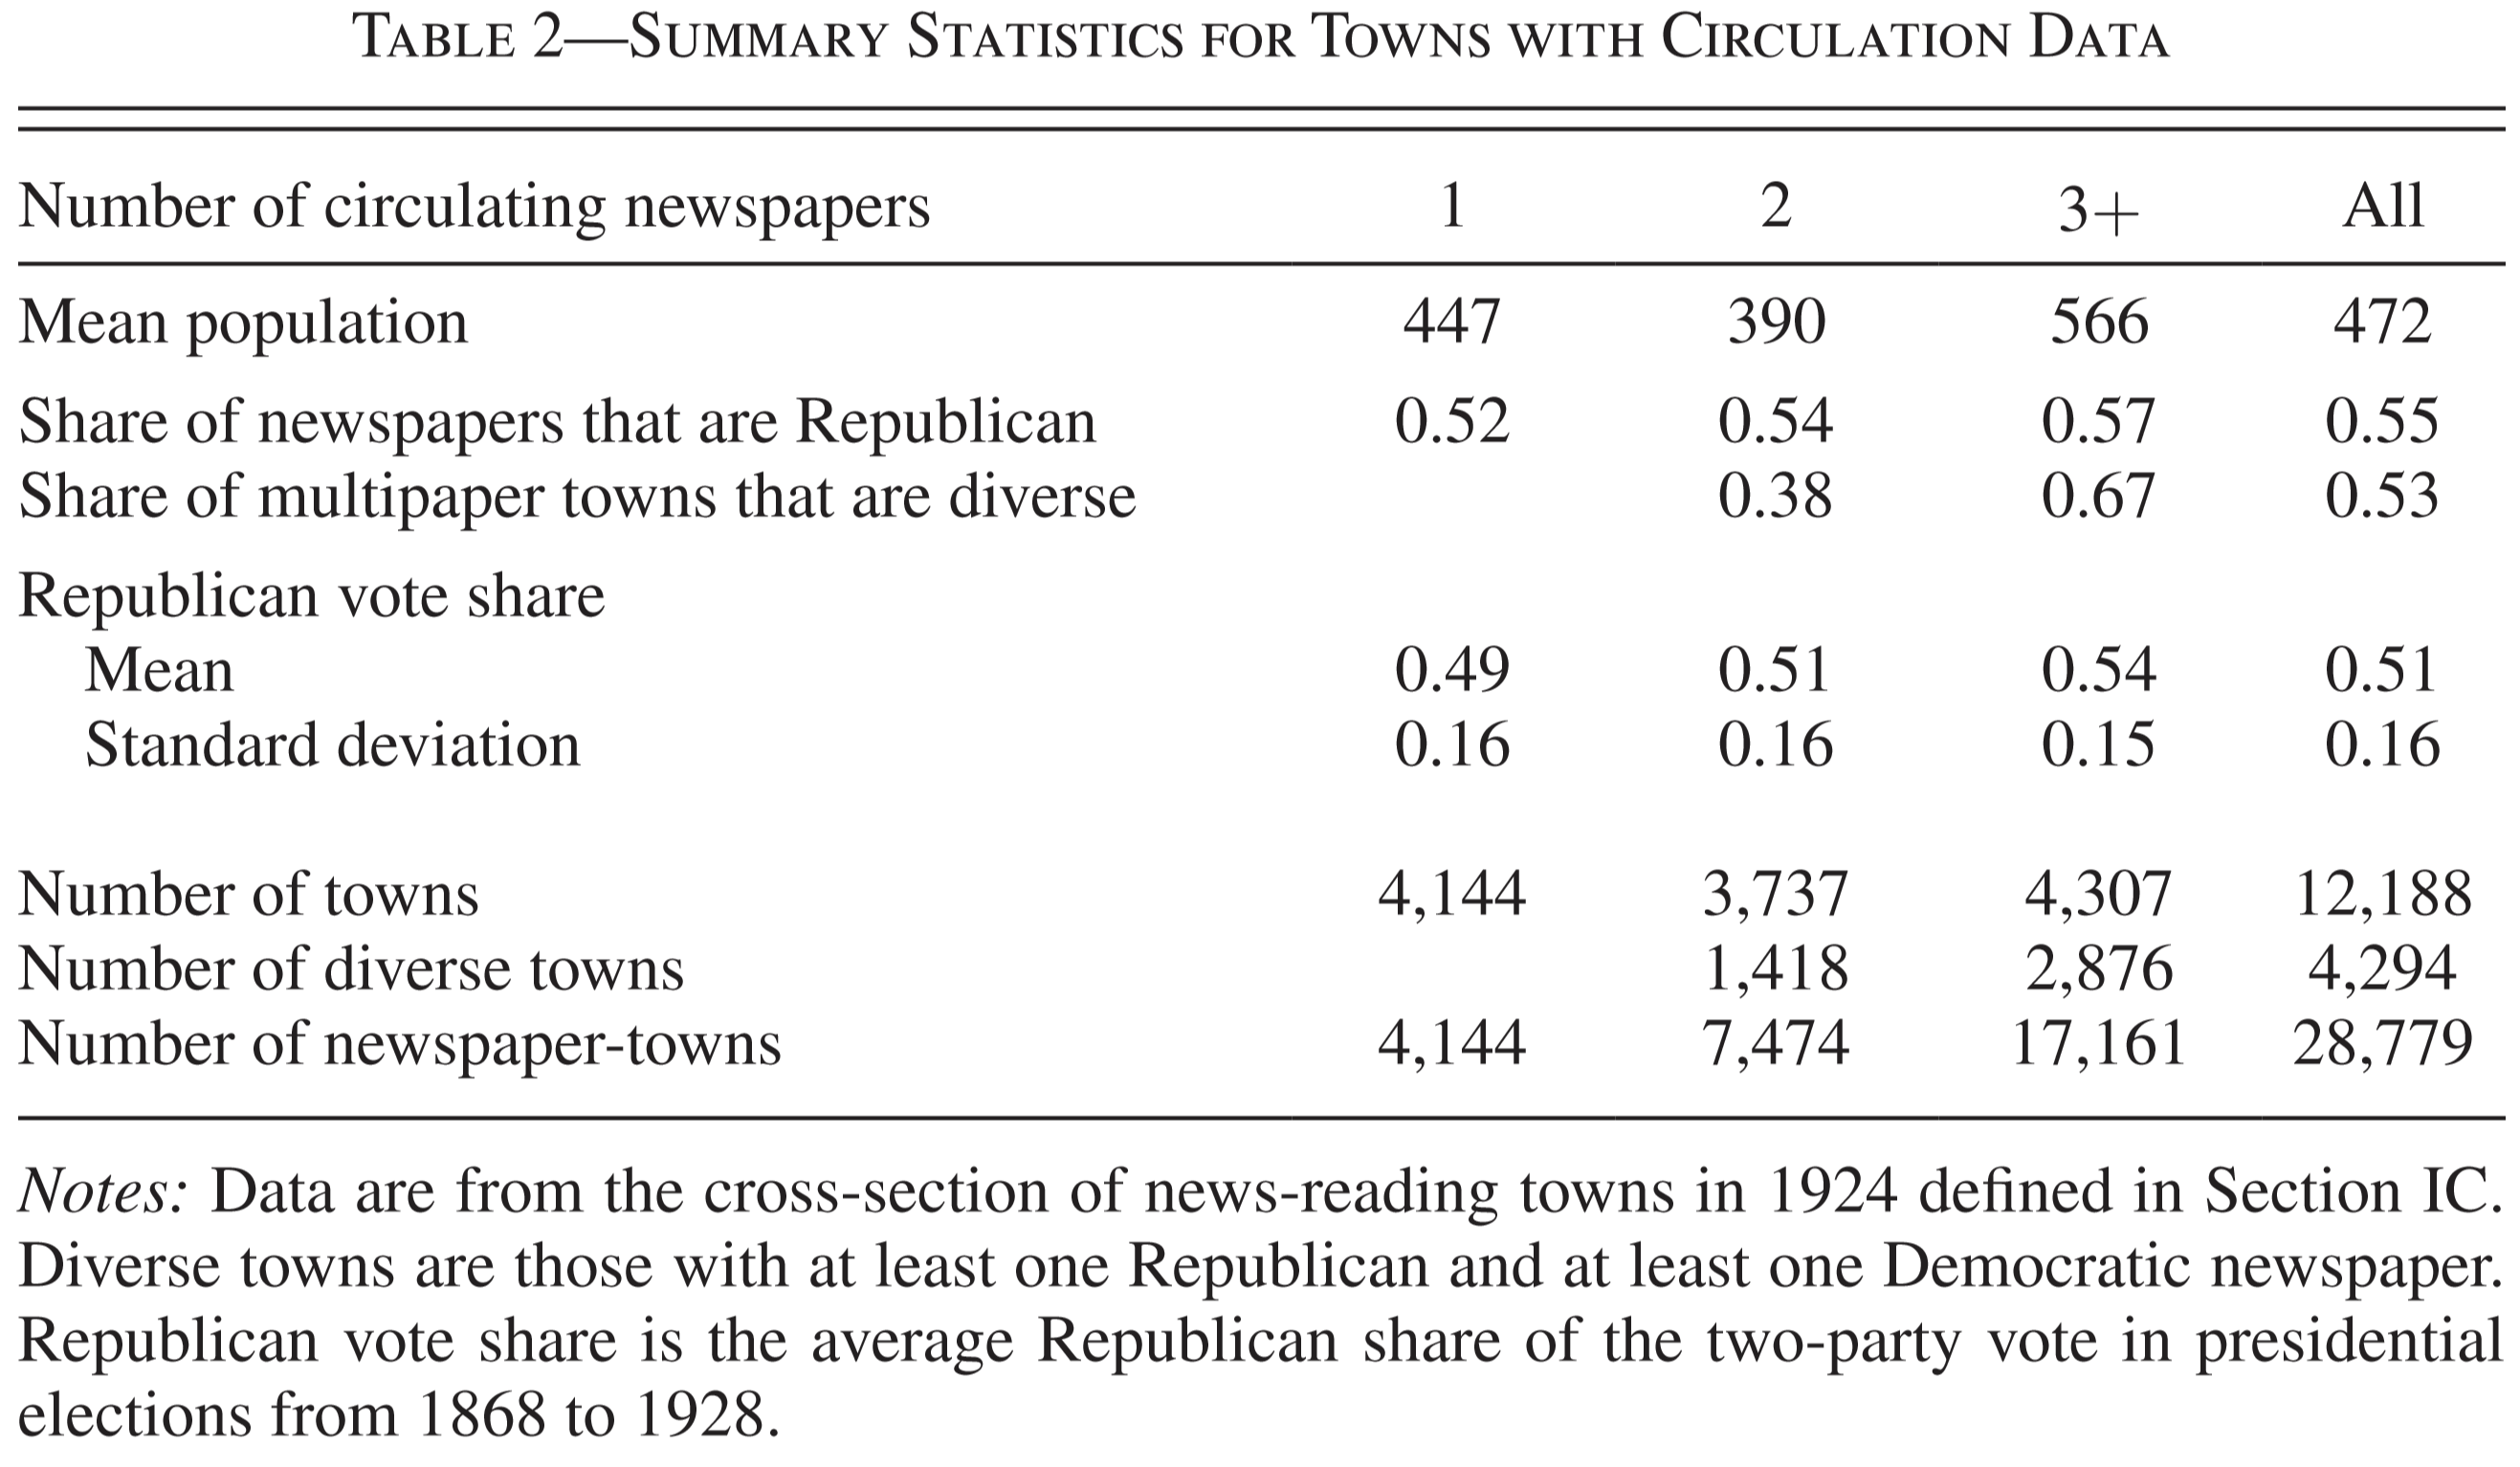
\includegraphics[scale=0.14]{Table2.png}
  \end{center}
  \end{figure}

  \begin{itemize}
    \item Mostly the same conclusions as before.
    \item Data lost by the matching process causing the share of Republican
      newspaper to fall to (55\%)
  \end{itemize}
  
\end{frame}

\begin{frame}[t]{Descriptive Evidence}
  \begin{itemize}
    \item Data shows that increasing the fraction Republican among voters 
      by 10 percentage points increases the relative circulation of Republican 
      papers by 10 percent.
    \item And that adding a second Republican paper to a market with one Republican and one Democratic newspaper reduces the relative circulation of the existing Republican paper by 4\%.
  \end{itemize}
\end{frame}

\begin{frame}[t]{Descriptive Evidence}
  \begin{figure}
  \begin{center}
    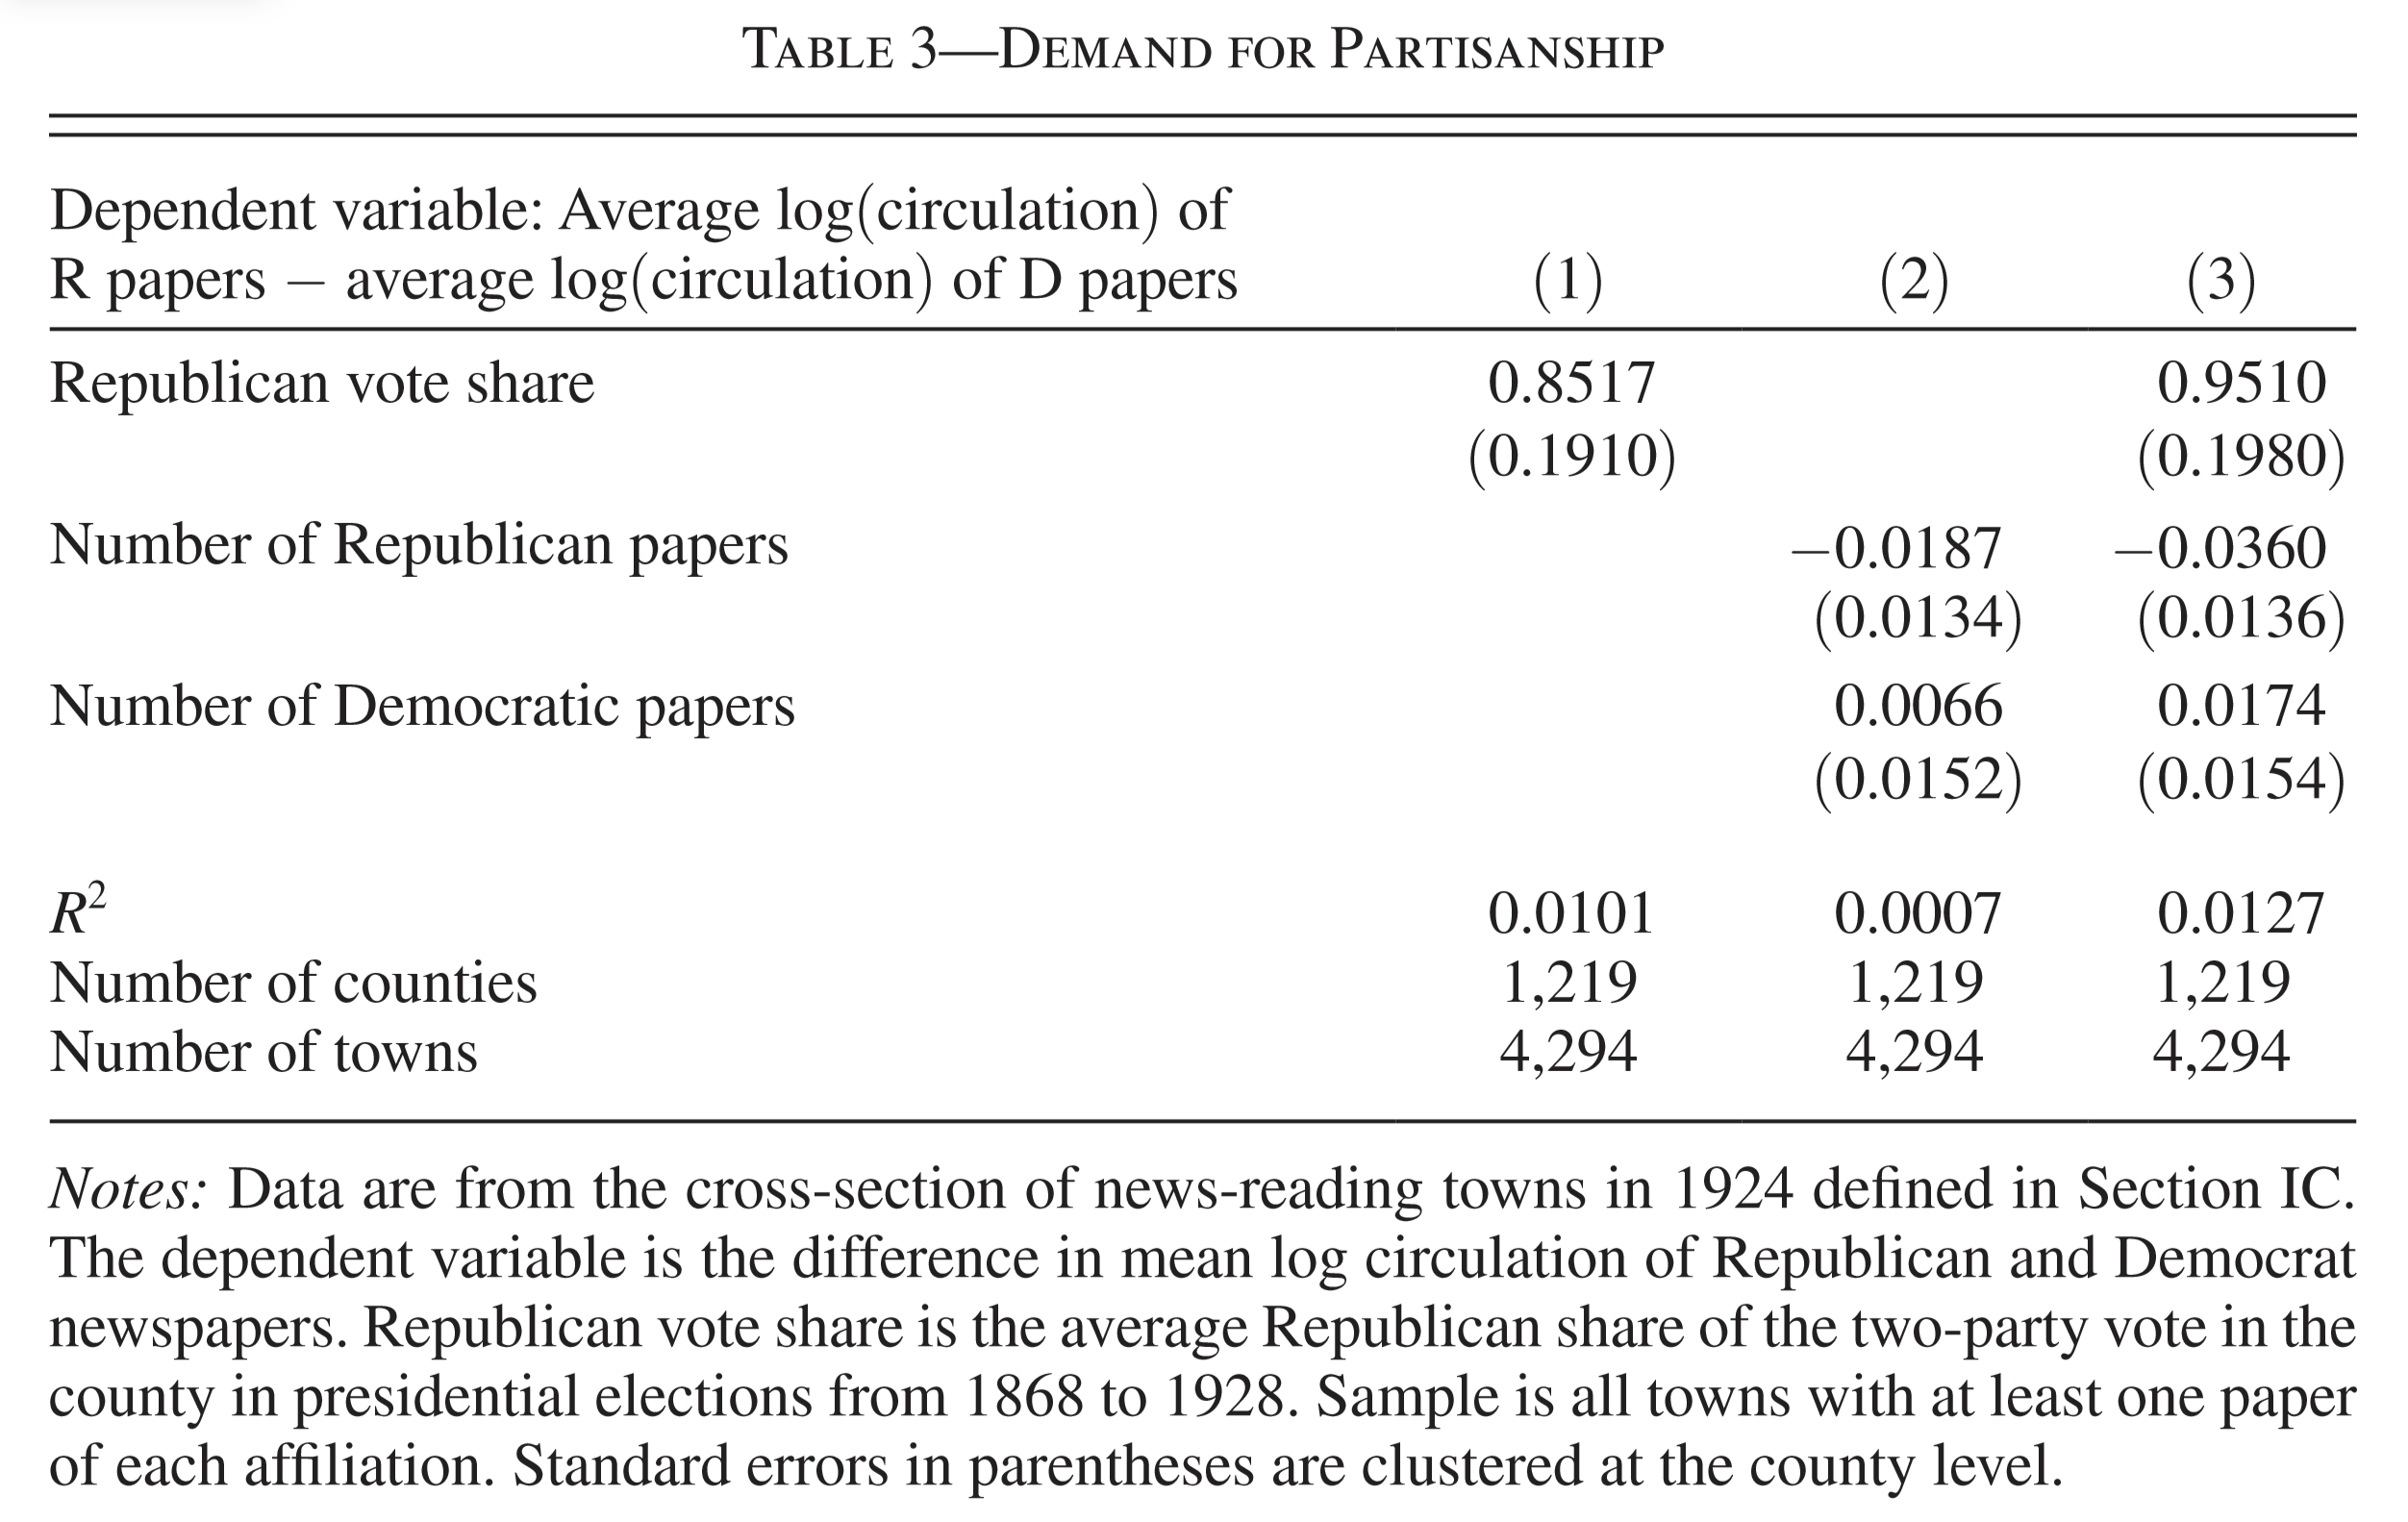
\includegraphics[scale=0.15]{Table3.png}
  \end{center}
  \end{figure}
\end{frame}

\begin{frame}[t]{Descriptive Evidence}
  \begin{itemize}
    \item Data shows that a 10 percentage point increase in the fraction of 
      Republican among the households increases the likelihood of a Republican 
      affiliation by 23\%
    \item But facing a Republican incumbent, instead of a Democratic one, 
      reduces the likelihood by 28\%.
  \end{itemize}
\end{frame}


\begin{frame}[t]{Descriptive Evidence}
  \begin{figure}
  \begin{center}
    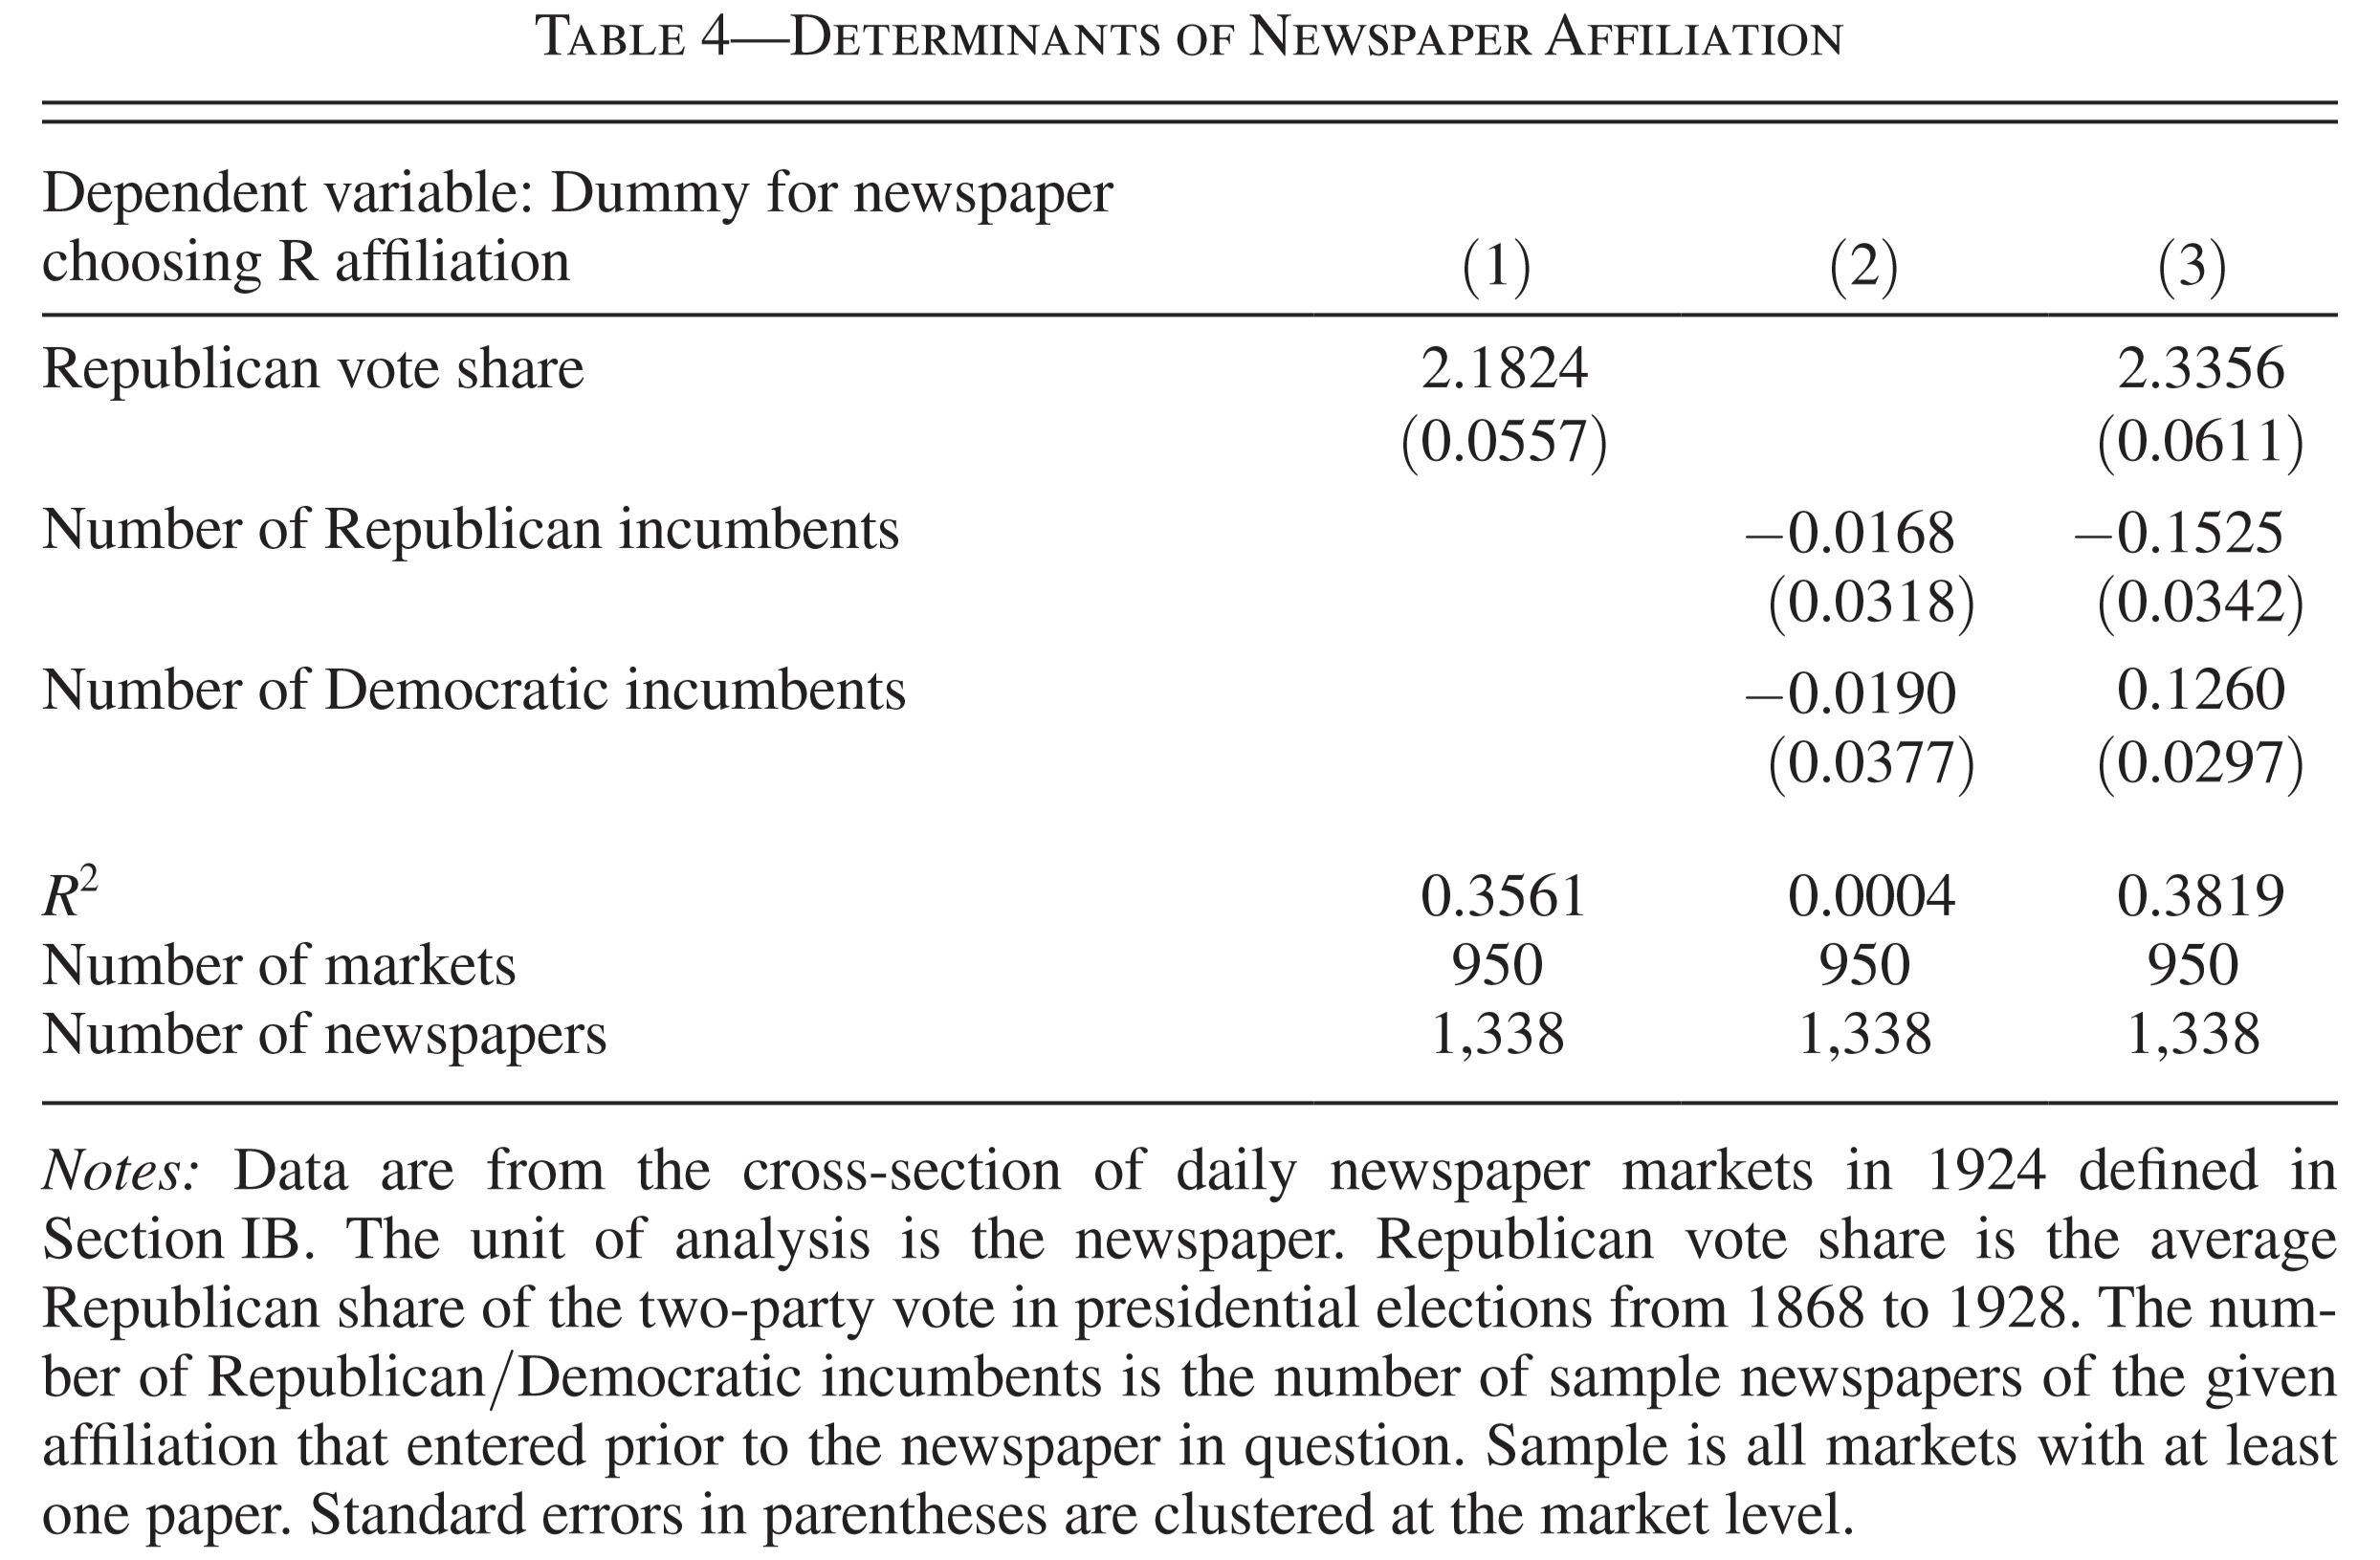
\includegraphics[scale=0.15]{Table4.png}
  \end{center}
  \end{figure}
\end{frame}

\begin{frame}[t]{Descriptive Evidence: Summary}
  \begin{figure}
  \begin{center}
    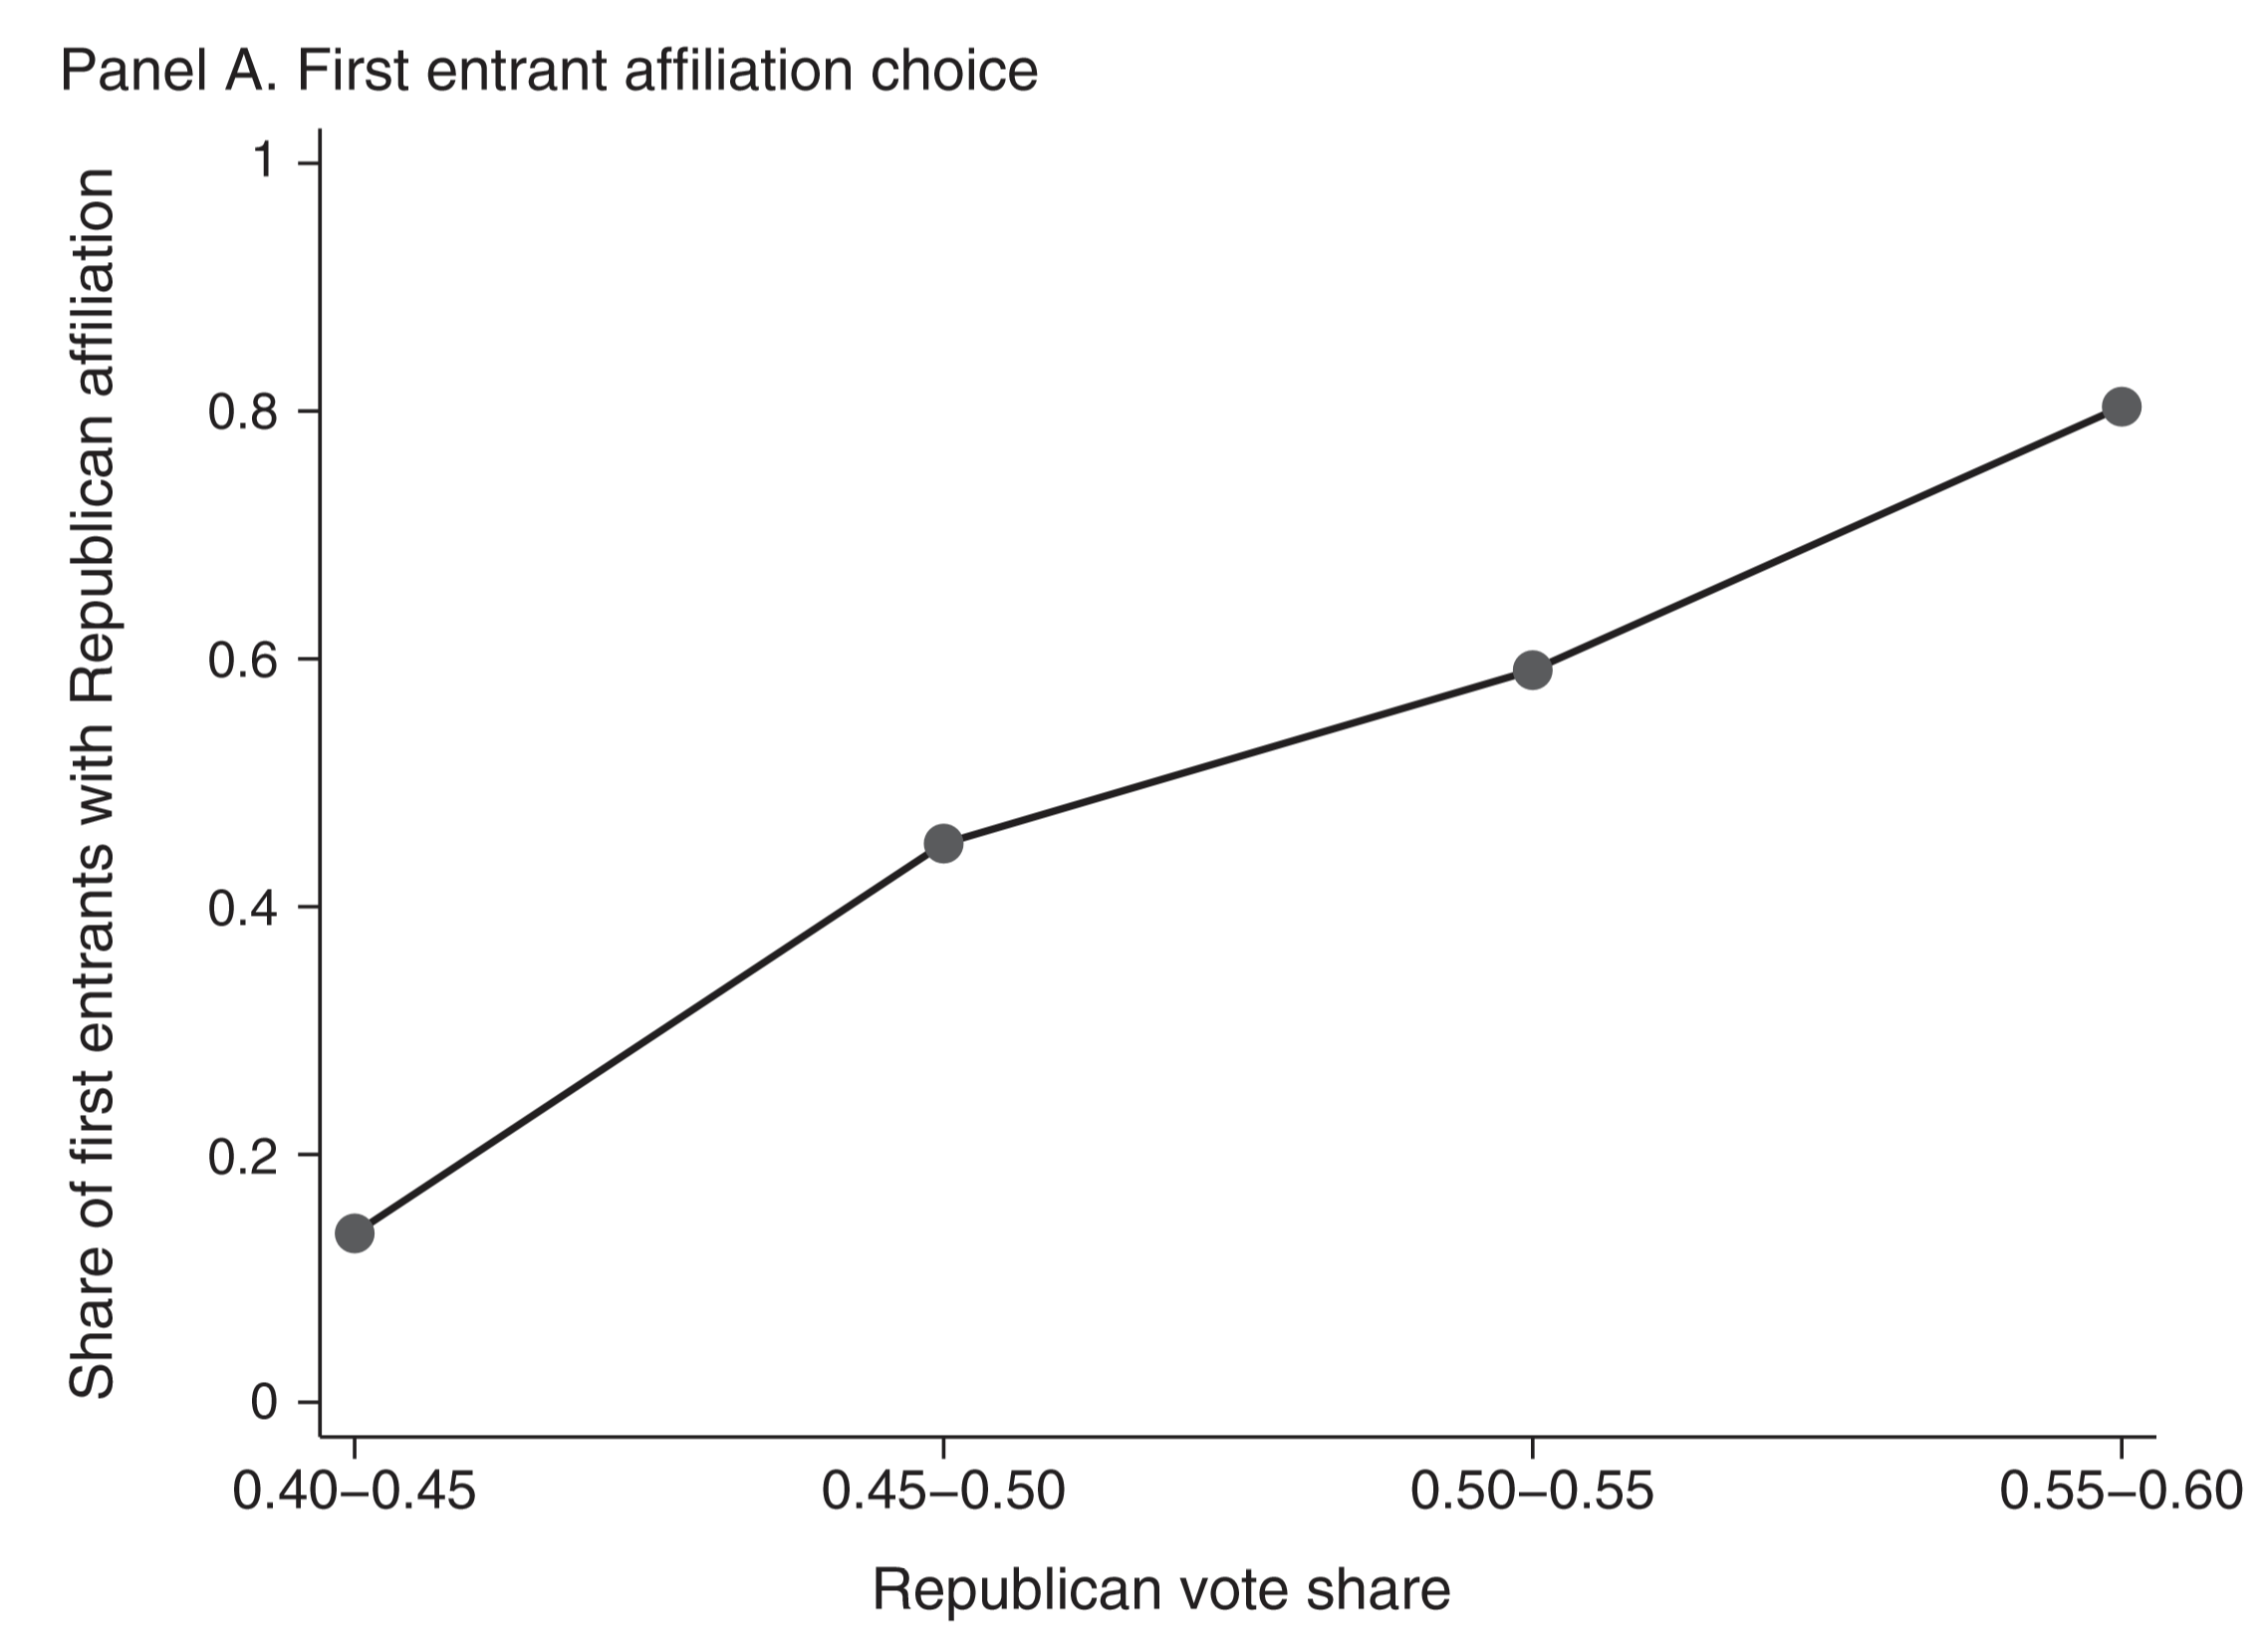
\includegraphics[scale=0.17]{Fig1A.png}
  \end{center}
  \end{figure}
\end{frame}

\begin{frame}[t]{Descriptive Evidence: Summary}
  \begin{figure}
  \begin{center}
    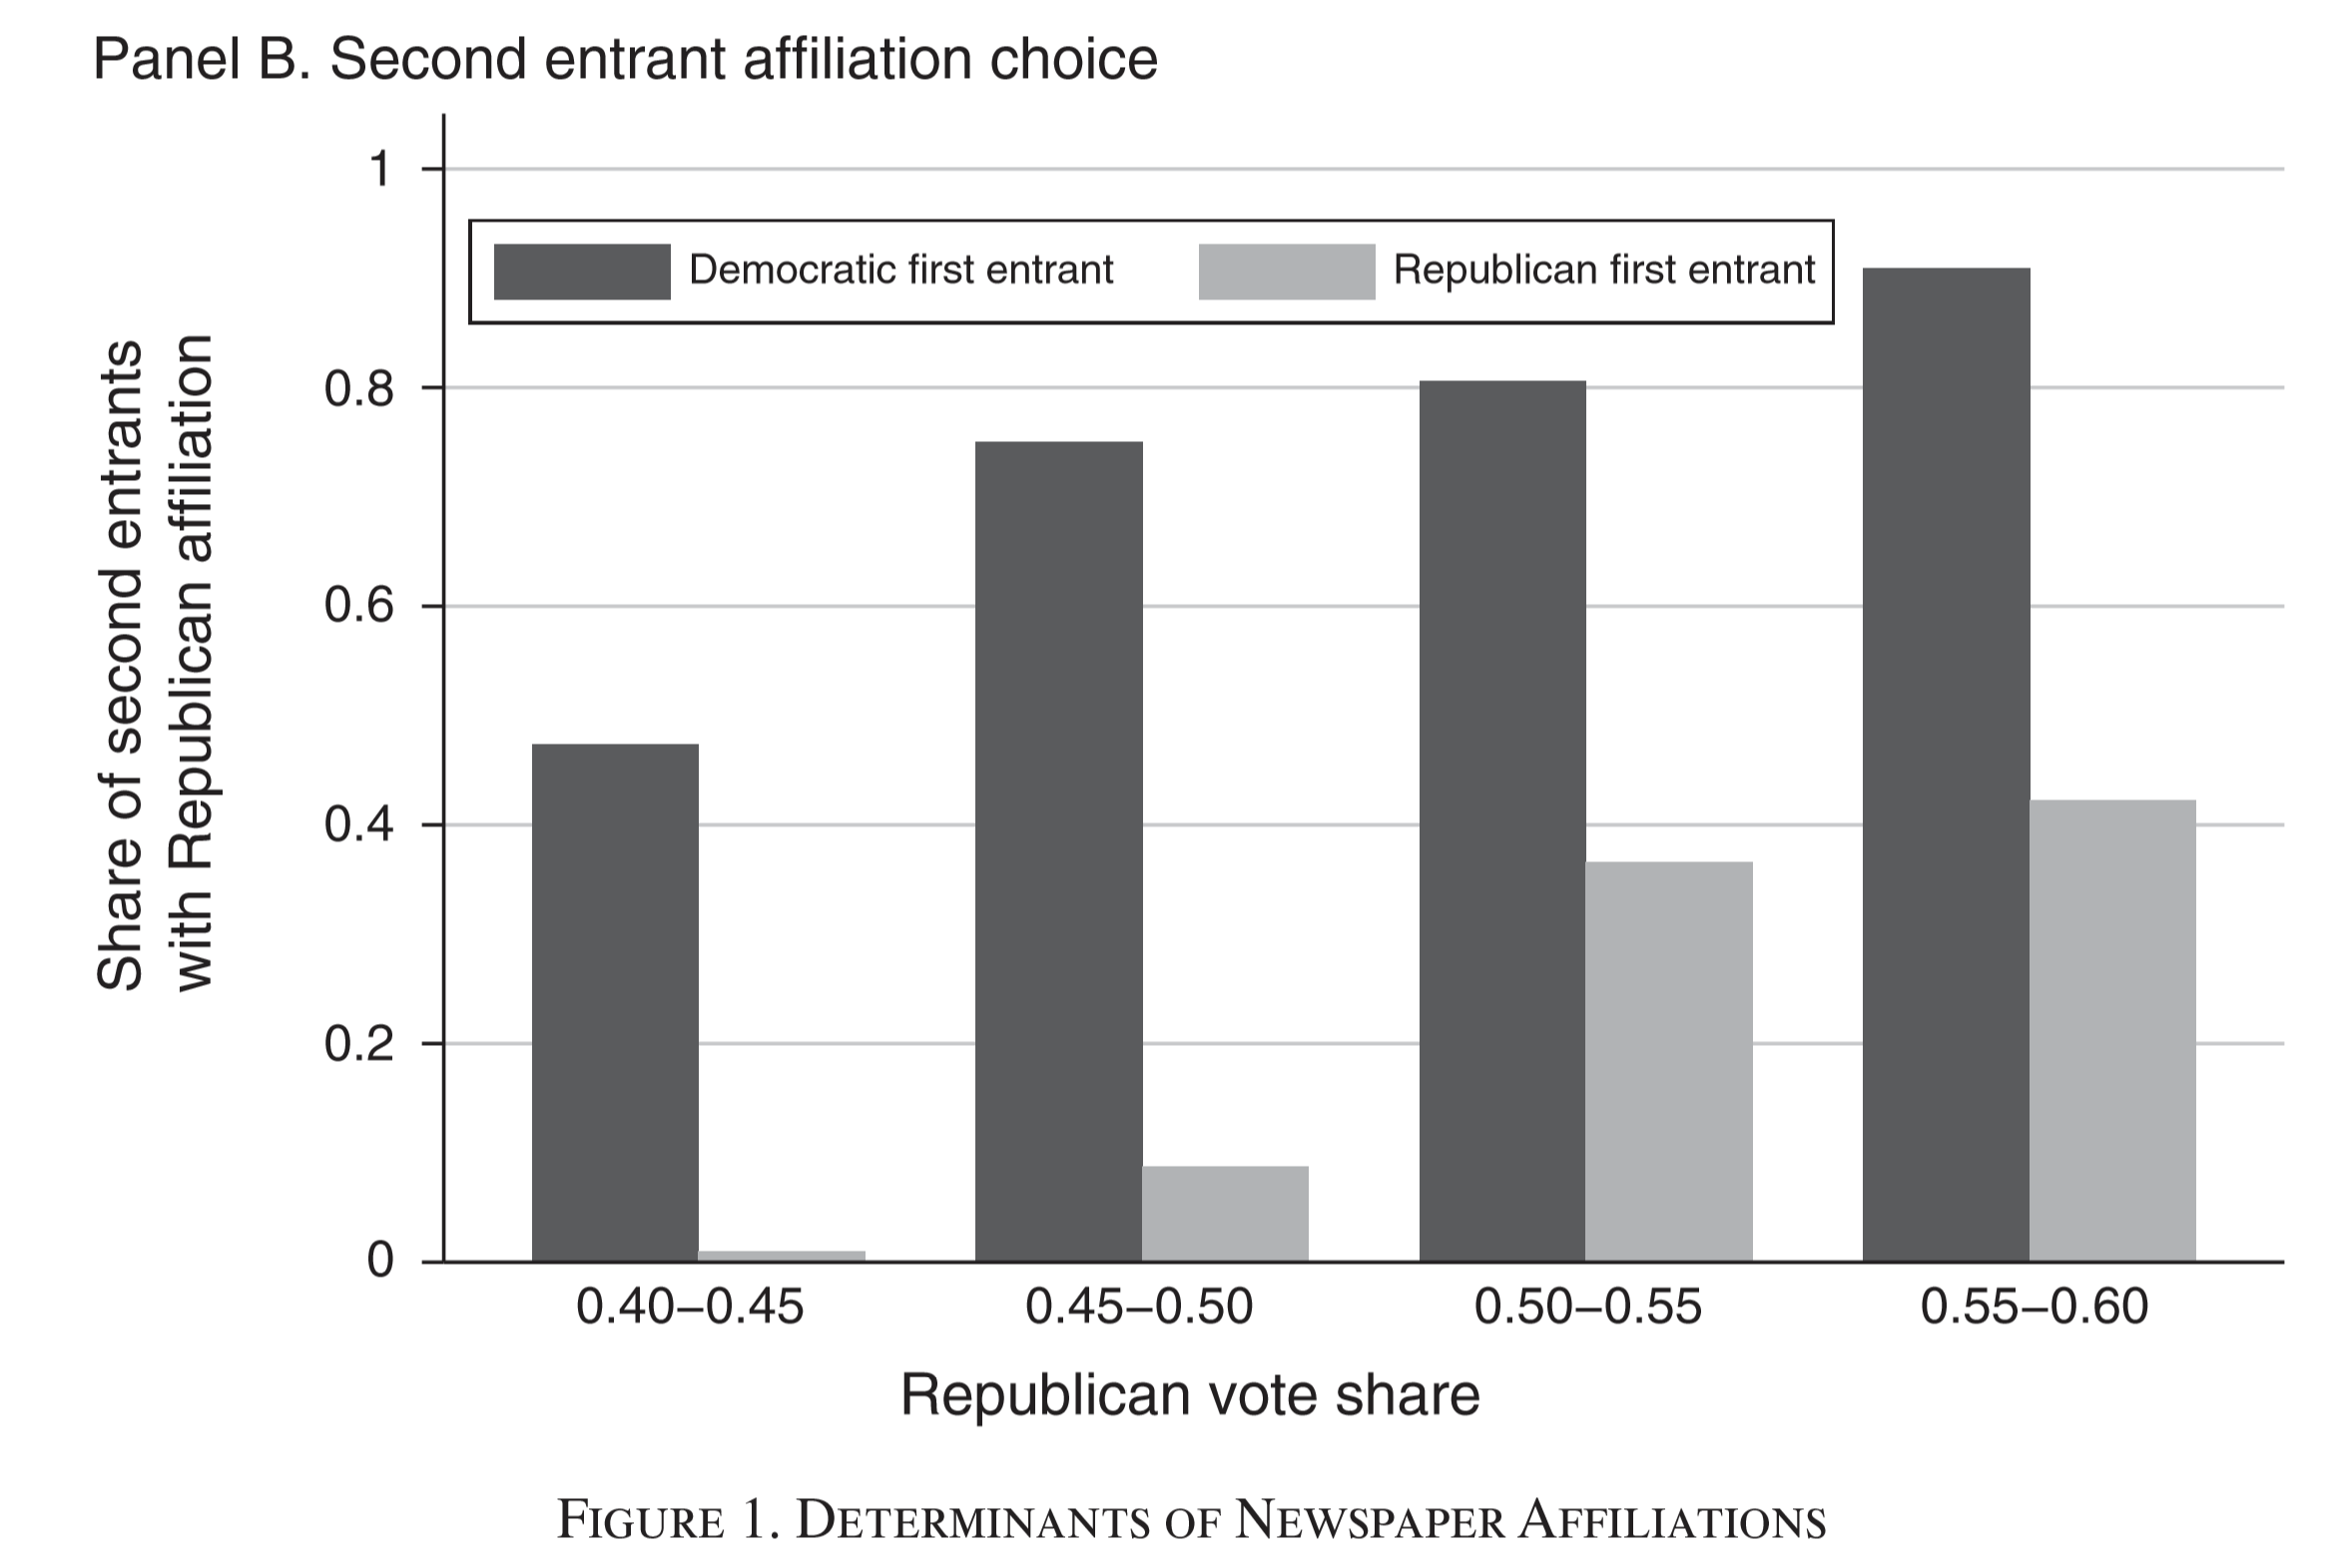
\includegraphics[scale=0.17]{Fig1B.png}
  \end{center}
  \end{figure}
\end{frame}

\begin{frame}[t]{Model Setup}
  \begin{itemize}
    \item There are $M$ markets. Each one is indexed by $m \in {1,...,M}$.
    \item Each market has a unit mas of homogeneous advertisers and a mass
      $S_m$ of households. Households are indexed by $i \in {1,...,S_m}$
    \item $J_m$ is the number of newspapers that choose to enter market $m$.
      Newspapers are indexed by $j \in {1,...,J_m}$.
    \item Each entering newspaper choose a political affiliation 
      $\tau_{jm} \in {R,D}.$
    \item Each household has a political affiliation $\theta_{im} \in {R, D}$.
    \item $\rho_m$ represents the share or Republican households within the 
      market and is common knowledge.
  \end{itemize}
\end{frame}
\end{document}
